\subsection{
    Линейные пространства. Определение, примеры.
}

\begin{definition}
    Непустое множество $\mathcal{L}$ называется \textbf{\textit{линейным пространством}} (афинным, векторным) над полем $\PP$, если $\forall \alpha, \beta \in \PP$ и $\forall \vec{a}, \vec{b} \in \mathcal{L}$ выполнены  линейность:  $(\alpha \vec{a} + \beta \vec{b}) \in \mathcal{L}$, и следующие аксиомы векторного пространства:

    \begin{enumerate}[nosep]
        \item $\vec{a} + \vec{b} = \vec{b} + \vec{a}$.
        \item $\forall \vec{c} \in \mathcal{L} \colon (\vec{a} + \vec{b}) + \vec{c} = \vec{a} + (\vec{b} + \vec{c})$.
        \item $\forall \vec{a} \thinspace \thinspace \exists \overrightarrow{0} \in \mathcal{L} \colon \vec{a} + \overrightarrow{0} = \vec{a}$.
        \item $\forall \vec{a} \thinspace \thinspace \exists \vec{a}' \in \mathcal{L} \colon \vec{a} + \vec{a'} = \overrightarrow{0}$.
        \item $(\alpha \beta) \vec{a} = \alpha(\beta \vec{a})$.
        \item $(\alpha + \beta)\vec{a} = \alpha \vec{a} + \beta \vec{a}$.
        \item $\alpha(\vec{a} + \vec{b}) = \alpha \vec{a} + \alpha \vec{b}$.
        \item $1 \cdot \vec{a} = \vec{a}$, $\forall \vec{a}$.
    \end{enumerate}
\end{definition}

\begin{definition}
    \textbf{\textit{Полем}} называется множество $\PP$ произвольной природы, на котором заданы две бинарные операции ($+$ и $\cdot$) и которое подчиняется следующим аксиомам:
    \begin{enumerate}[nosep]
        \item $\vec{a} + \vec{b} = \vec{b} + \vec{a}$.
        \item $\forall \vec{c} \colon (\vec{a} + \vec{b}) + \vec{c} = \vec{a} + (\vec{b} + \vec{c})$.
        \item $\forall \vec{a} \thinspace \thinspace \exists \overrightarrow{0} \in \PP \colon \vec{a} + \overrightarrow{0} = \vec{a}$.
        \item $\forall \vec{a} \thinspace \thinspace \exists \vec{a}' \in \PP \colon \vec{a} + \vec{a'} = \overrightarrow{0}$.
        \item $\vec{a} \cdot \vec{b} = \vec{b} \cdot \vec{a}$.
        \item $(\vec{a} \cdot \vec{b}) \cdot \vec{c} = \vec{a} \cdot (\vec{b} \cdot \vec{c})$.
        \item $\forall \vec{a} \thinspace \thinspace \exists \vec{e} \in \PP \thinspace \text{(\textbf{единичный})} \colon \vec{a} \cdot \vec{e} = \vec{a}$.
        \item $\forall \vec{a} \in \PP, \vec{a} \ne \vec{0} \thinspace \thinspace \exists \vec{a}^{-1} \in \PP \thinspace \colon \vec{a} \cdot \vec{a}^{-1} = \vec{e}$.
        \item $(\vec{a} + \vec{b}) \cdot \vec{c} = (\vec{a} \cdot \vec{c}) + (\vec{b} \cdot \vec{c})$.
    \end{enumerate}
\end{definition}

\begin{definition}
    Элементы линейного пространства называются (абстрактными) \textbf{\textit{векторами}}.
\end{definition}

\begin{example}~
    \begin{itemize}[nosep]
        \item множество $\mathcal{V}_3 (\mathcal{V}_2)$ всех \textit{свободных векторов} в пространстве (на плоскости) с линейными операциями над векторами - линейное пространство.
        
        \item множество всех \textit{геометрических векторов} в пространстве с началом в данной точке и параллельных данной плоскости (рис. \ref{fig:picture_02_1}) с линейными операциями над векторами.
        \begin{figure}[H]
            \centering
            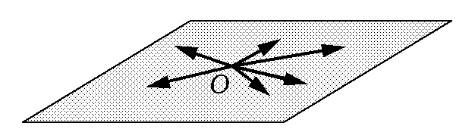
\includegraphics[scale=0.5]{images/module1/question02/1.jpg}
            \label{fig:picture_02_1}
            \caption{}
        \end{figure}

        \item множество $M_{mn}(\RR)$ матриц типа $m \times n$, элементами которых являются действительные числа, с линейными операциями над матрицами.

        \item множество $K_n[x]$ многочленов переменного $x$ степени, не превышающей $n$, которые как функции можно складывать и умножать на действительные числа.

        \item множество всех решений данной ОСЛАУ (решения можно рассматривать как матрицы-столбцы, складывать и умножать на числа по законам матричных операций).

        \item множество функций, непрерывных на отрезке, с обычными операциями сложения функций и умножения функции на число.

        \item $\RR$ является линейным пространством над полем $\QQ$.
        
        \item $\CC$ является линейным пространством над полем $\RR$.
    \end{itemize}
\end{example}
